% fig2_mediacao.tex — Decomposição da Mediação da Informalidade
% Compilar standalone via: pdflatex fig2_mediacao.tex
\documentclass[border=6pt]{standalone}
\usepackage[T1]{fontenc}
\usepackage[utf8]{inputenc}
\usepackage{amsmath,amssymb}
\usepackage{tikz}
\usetikzlibrary{arrows.meta,calc}

% Paleta Institucional
\definecolor{instblue}{HTML}{012169}
\definecolor{instgold}{HTML}{B9975B}
\definecolor{vermillion}{HTML}{D55E00}
\definecolor{gridgray}{HTML}{E5E5E5}
\definecolor{axisgray}{HTML}{333333}

\begin{document}
% Coordinate map:
% x represents AI exposure [0, 10], scale: X(x) = x * 1.15 cm -> range [0, 11.5] cm
% y represents informality pct [0, 100], scale: Y(y) = y * 0.055 cm -> range [0, 5.5] cm
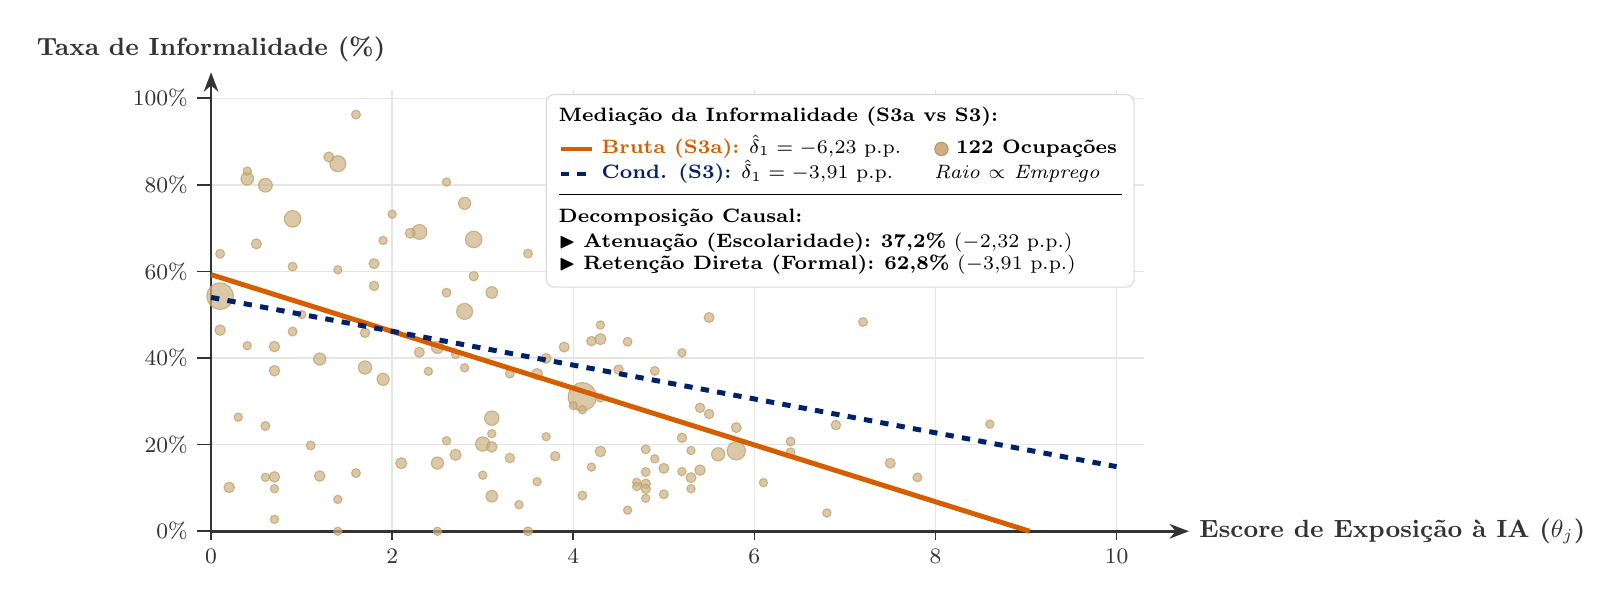
\begin{tikzpicture}[x=1.15cm, y=0.055cm]

  % Background grid lines
  \foreach \x in {0, 2, 4, 6, 8, 10} {
    \draw[gridgray, line width=0.5pt] (\x, 0) -- (\x, 102);
    \draw[axisgray, line width=0.6pt] (\x, 0) -- (\x, -2);
    \node[below, font=\footnotesize, text=axisgray] at (\x, -2) {\x};
  }

  \foreach \y in {0, 20, 40, 60, 80, 100} {
    \draw[gridgray, line width=0.5pt] (0, \y) -- (10.3, \y);
    \draw[axisgray, line width=0.6pt] (0, \y) -- (-0.15, \y);
    \node[left, font=\footnotesize, text=axisgray] at (-0.15, \y) {\y\%};
  }

  % Axes
  \draw[axisgray, line width=0.9pt, ->, >=Stealth] (0, 0) -- (10.8, 0) node[right, font=\small\bfseries, text=axisgray] {Escore de Exposição à IA ($\theta_j$)};
  \draw[axisgray, line width=0.9pt, ->, >=Stealth] (0, 0) -- (0, 106) node[above, font=\small\bfseries, text=axisgray] {Taxa de Informalidade (\%)};

  % Scatter points of 122 occupations (X = exposure, Y = informality, radius proportional to employment)
  \foreach \px/\py/\pr in {
    4.10/31.06/5.1, 0.10/54.30/4.8, 5.80/18.58/3.3, 2.90/67.39/3.0, 0.90/72.15/3.0, 
    2.80/50.77/2.9, 1.40/84.88/2.9, 2.30/69.12/2.7, 3.10/26.12/2.6, 3.00/20.15/2.6, 
    0.60/79.91/2.5, 1.70/37.82/2.4, 5.60/17.76/2.4, 0.40/81.42/2.3, 2.50/15.75/2.2, 
    1.20/39.77/2.2, 1.90/35.08/2.2, 2.80/75.72/2.2, 2.50/42.47/2.2, 3.10/55.15/2.1, 
    3.10/8.09/2.1, 4.30/44.38/2.0, 3.60/36.31/2.0, 2.70/17.65/2.0, 2.10/15.71/2.0, 
    1.20/12.75/1.9, 4.30/18.42/1.9, 0.10/46.45/1.9, 0.70/42.66/1.9, 0.20/10.12/1.9, 
    0.70/12.56/1.9, 0.70/37.07/1.9, 5.40/14.12/1.9, 3.10/19.49/1.9, 5.80/23.95/1.8, 
    1.80/61.80/1.8, 5.30/12.38/1.8, 2.20/68.83/1.8, 5.50/49.37/1.8, 2.30/41.34/1.8, 
    0.50/66.38/1.8, 3.70/39.91/1.8, 5.00/14.53/1.8, 7.50/15.72/1.8, 3.90/42.54/1.8, 
    1.30/86.44/1.8, 3.30/16.92/1.7, 1.80/56.66/1.7, 1.70/45.83/1.7, 5.50/27.09/1.7, 
    4.20/43.91/1.7, 6.90/24.52/1.7, 5.20/21.57/1.7, 3.80/17.33/1.7, 2.90/58.91/1.7, 
    5.40/28.52/1.7, 4.80/10.97/1.7, 4.80/9.82/1.7, 4.50/37.33/1.7, 2.60/55.10/1.6, 
    6.40/20.73/1.6, 0.90/46.12/1.6, 3.50/64.13/1.6, 4.10/8.25/1.6, 4.80/18.91/1.6, 
    7.80/12.44/1.6, 0.10/64.08/1.6, 3.50/0.00/1.6, 1.10/19.82/1.6, 1.60/13.44/1.6, 
    5.00/8.54/1.6, 4.90/37.03/1.6, 0.60/24.32/1.6, 0.90/61.12/1.6, 3.30/36.42/1.6, 
    6.40/18.23/1.6, 4.80/13.68/1.6, 4.60/43.76/1.6, 1.60/96.22/1.6, 7.20/48.33/1.6, 
    1.00/50.04/1.5, 3.60/11.45/1.5, 4.20/14.83/1.5, 2.60/20.89/1.5, 0.60/12.46/1.5, 
    2.40/36.93/1.5, 4.80/60.39/1.5, 4.30/30.81/1.5, 2.60/80.65/1.5, 4.90/16.73/1.5, 
    4.70/11.31/1.5, 5.20/41.22/1.5, 4.60/4.88/1.5, 5.30/18.66/1.5, 2.70/40.85/1.5, 
    0.70/2.75/1.5, 4.90/64.38/1.5, 6.10/11.23/1.5, 6.80/4.22/1.5, 2.80/37.75/1.5, 
    4.10/28.07/1.5, 3.10/22.54/1.5, 4.80/7.62/1.5, 0.30/26.35/1.5, 3.40/6.14/1.5, 
    5.20/13.79/1.5, 0.70/9.82/1.5, 2.00/73.23/1.5, 1.40/0.00/1.5, 0.40/42.85/1.5, 
    3.70/21.84/1.5, 1.40/7.35/1.5, 4.00/29.00/1.5, 3.00/12.95/1.5, 4.70/10.33/1.5, 
    5.30/9.83/1.5, 4.30/47.64/1.5, 0.40/83.19/1.5, 2.50/0.00/1.5, 8.60/24.74/1.5, 
    1.90/67.15/1.5, 1.40/60.39/1.5
  } {
    \filldraw[fill=instgold!75, draw=instgold!95, line width=0.4pt, opacity=0.7] (\px, \py) circle (\pr pt);
  }

  % Regression Lines:
  % S3a (Bruta): y = 59.27 - 6.55 x -> x = 0: y = 59.27; x = 9.04: y = 0
  \draw[vermillion, line width=1.8pt] (0, 59.27) -- (9.04, 0);

  % S3 (Líquida / Condicional à Escolaridade): y = 54.0 - 3.9068 x -> x = 0: y = 54.0; x = 10: y = 14.93
  \draw[instblue, line width=1.8pt, dashed] (0, 54.0) -- (10.0, 14.93);

  % Statistics and Decomposition Card at Top Right (x in [4.0, 10.2], y in [62, 101])
  \node[draw=gray!30, fill=white, rounded corners=3pt, inner sep=4.5pt, anchor=north east] at (10.2, 101) {
    \begin{minipage}{7.15cm}
      \scriptsize
      \textbf{Mediação da Informalidade (S3a vs S3):}\\[2pt]
      \begin{tabular}{@{}l@{\hspace{12pt}}l@{}}
        \tikz[baseline=-0.5ex]\draw[vermillion, line width=1.4pt] (0,0)--(0.35,0); \textcolor{vermillion}{\textbf{Bruta (S3a):}} $\hat{\delta}_1 = -6{,}23$ p.p. & \tikz[baseline=-0.5ex]\filldraw[fill=instgold!75,draw=instgold] (0,0) circle (2.4pt); \textbf{122 Ocupações} \\
        \tikz[baseline=-0.5ex]\draw[instblue, line width=1.4pt, dashed] (0,0)--(0.35,0); \textcolor{instblue}{\textbf{Cond. (S3):}} $\hat{\delta}_1 = -3{,}91$ p.p. & \textit{Raio $\propto$ Emprego}
      \end{tabular}\\[3pt]
      \rule{\linewidth}{0.3pt}\\[2pt]
      \textbf{Decomposição Causal:}\\[1pt]
      $\blacktriangleright$ \textbf{Atenuação (Escolaridade):} \textbf{37,2\%} ($-2{,}32$ p.p.)\\
      $\blacktriangleright$ \textbf{Retenção Direta (Formal):} \textbf{62,8\%} ($-3{,}91$ p.p.)
    \end{minipage}
  };

\end{tikzpicture}
\end{document}
